\section{Stator Re-design}
\label{AppendixA}
This appendix is used for the simulation images of the re-design and an alternative 
\subsection{Shut-down condition}

\begin{figure}[H]
\centering
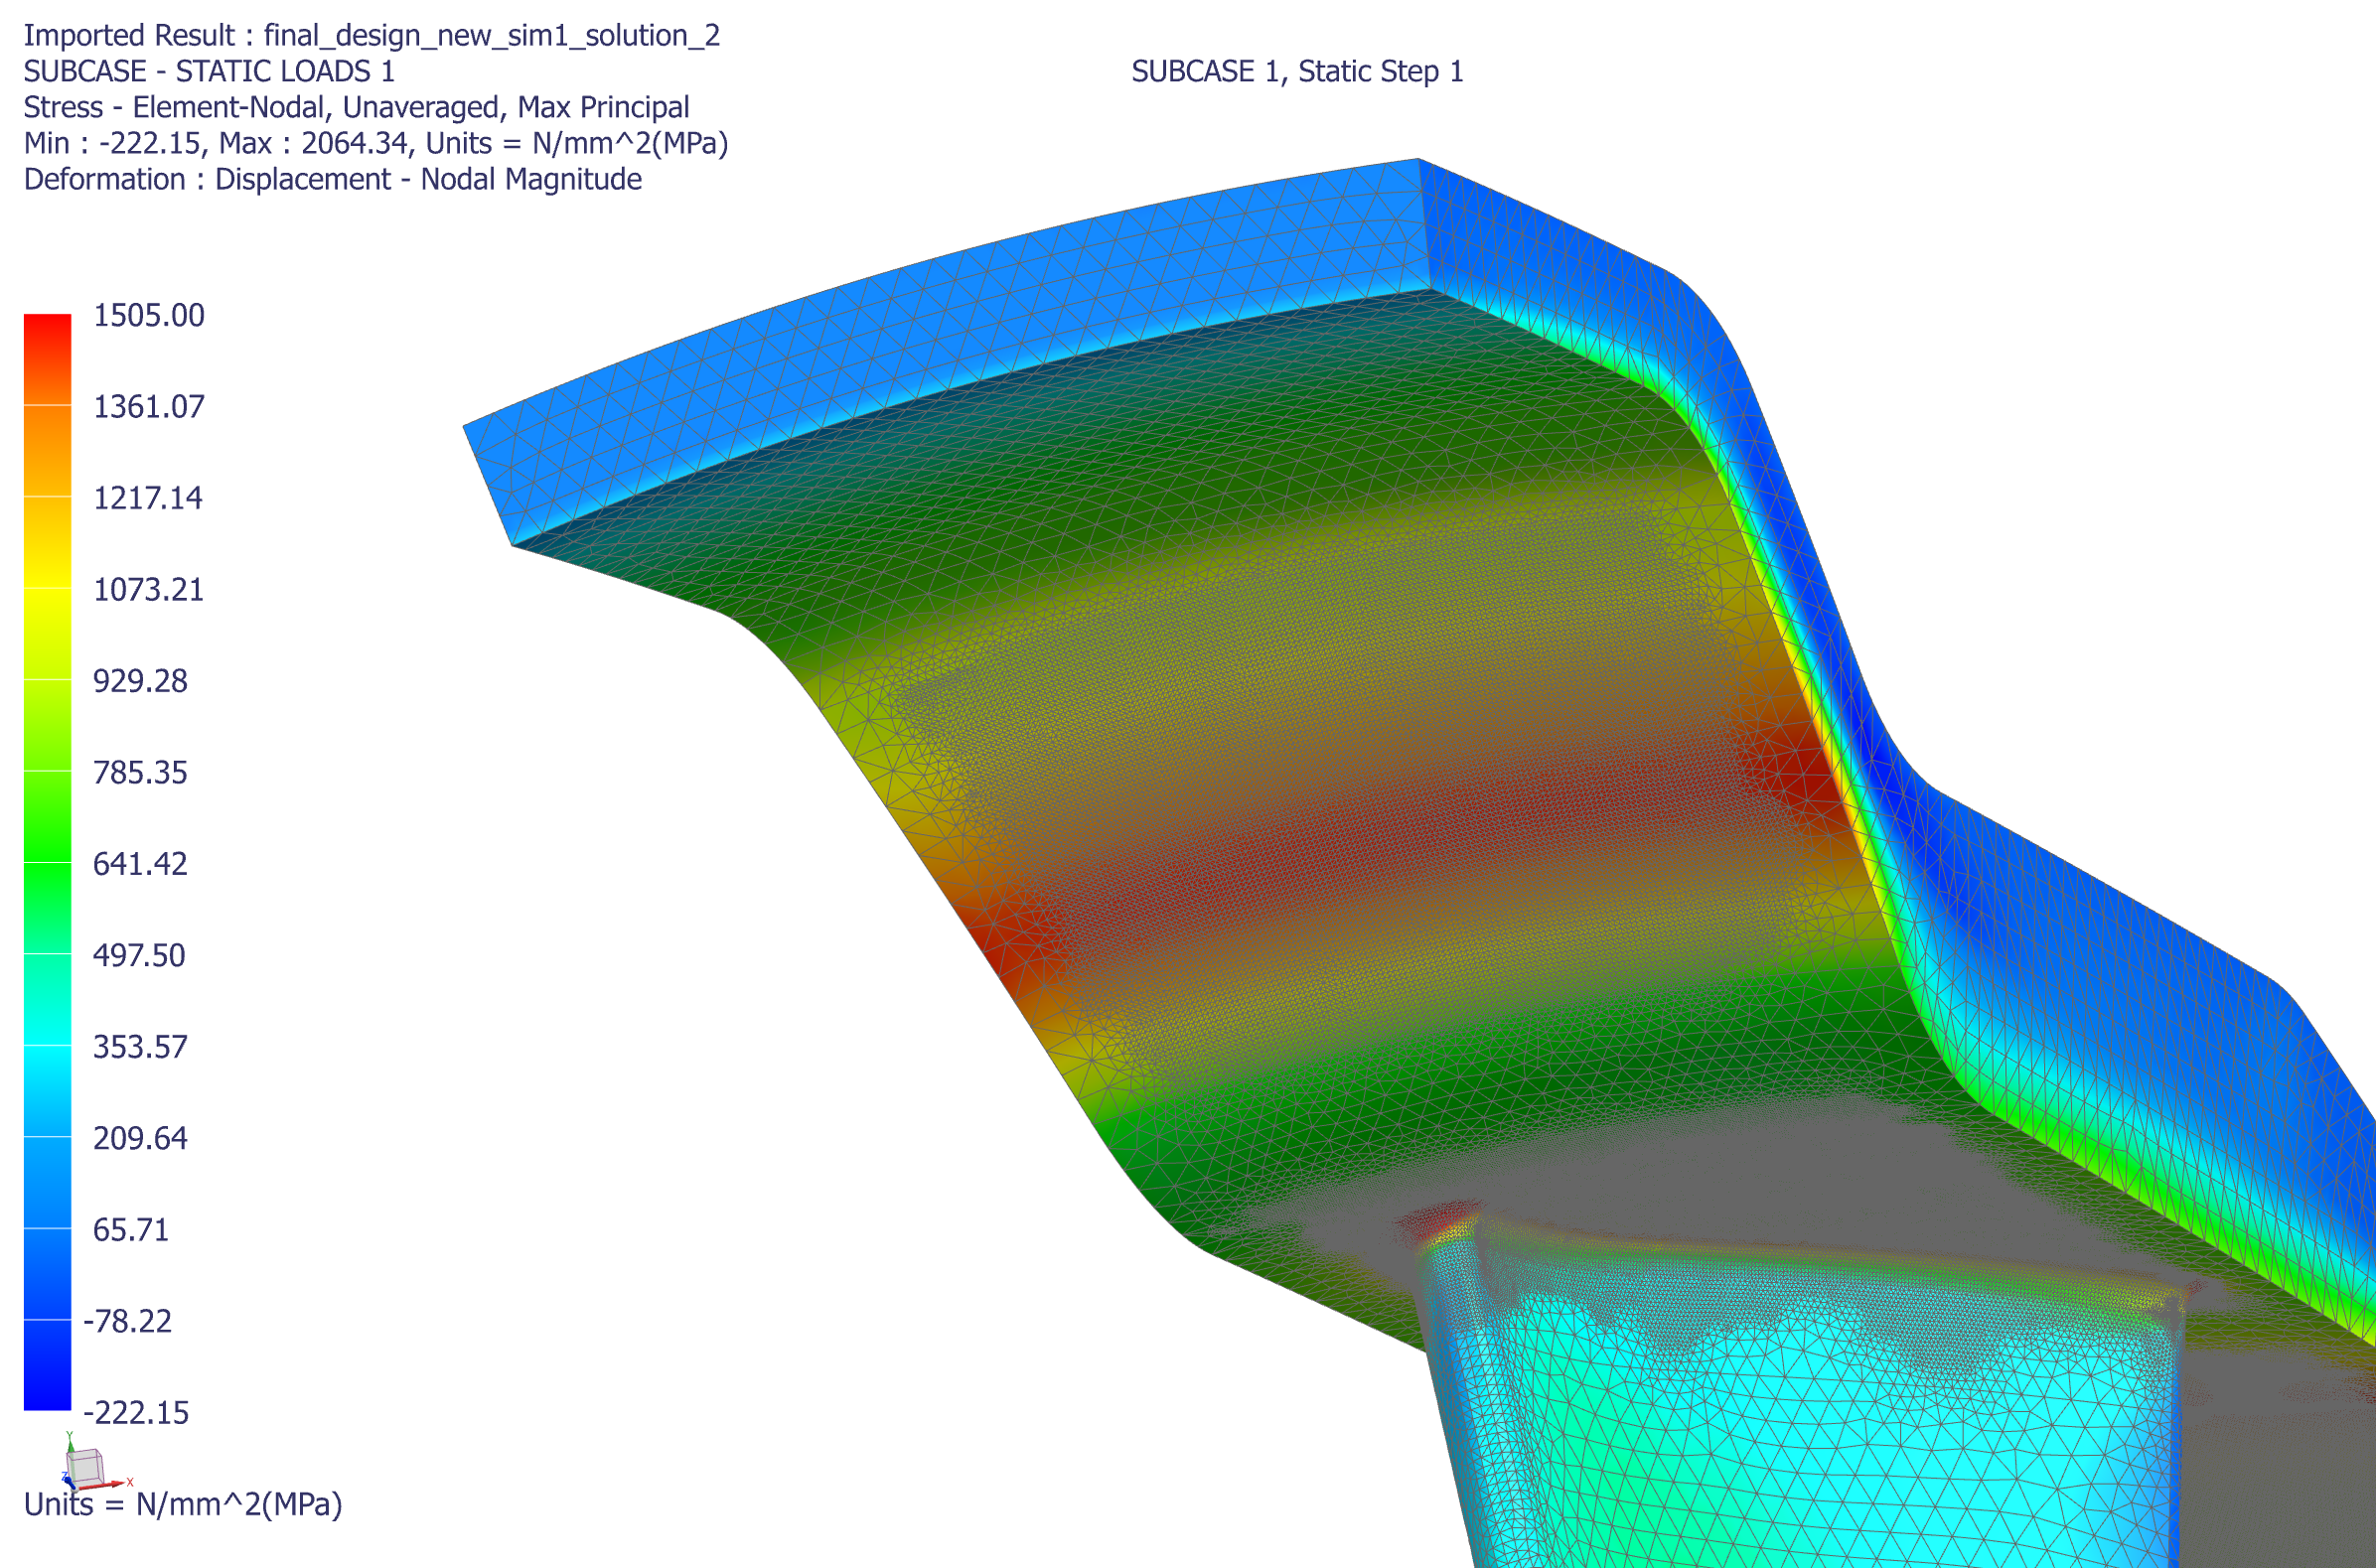
\includegraphics[width=0.7\textwidth]{Figures/finaldesign_shutdown1.png}
\caption{High stress point Shut-down condition}
\label{fig:highstressshutdownl}
\end{figure}

\begin{figure}[H]
\centering
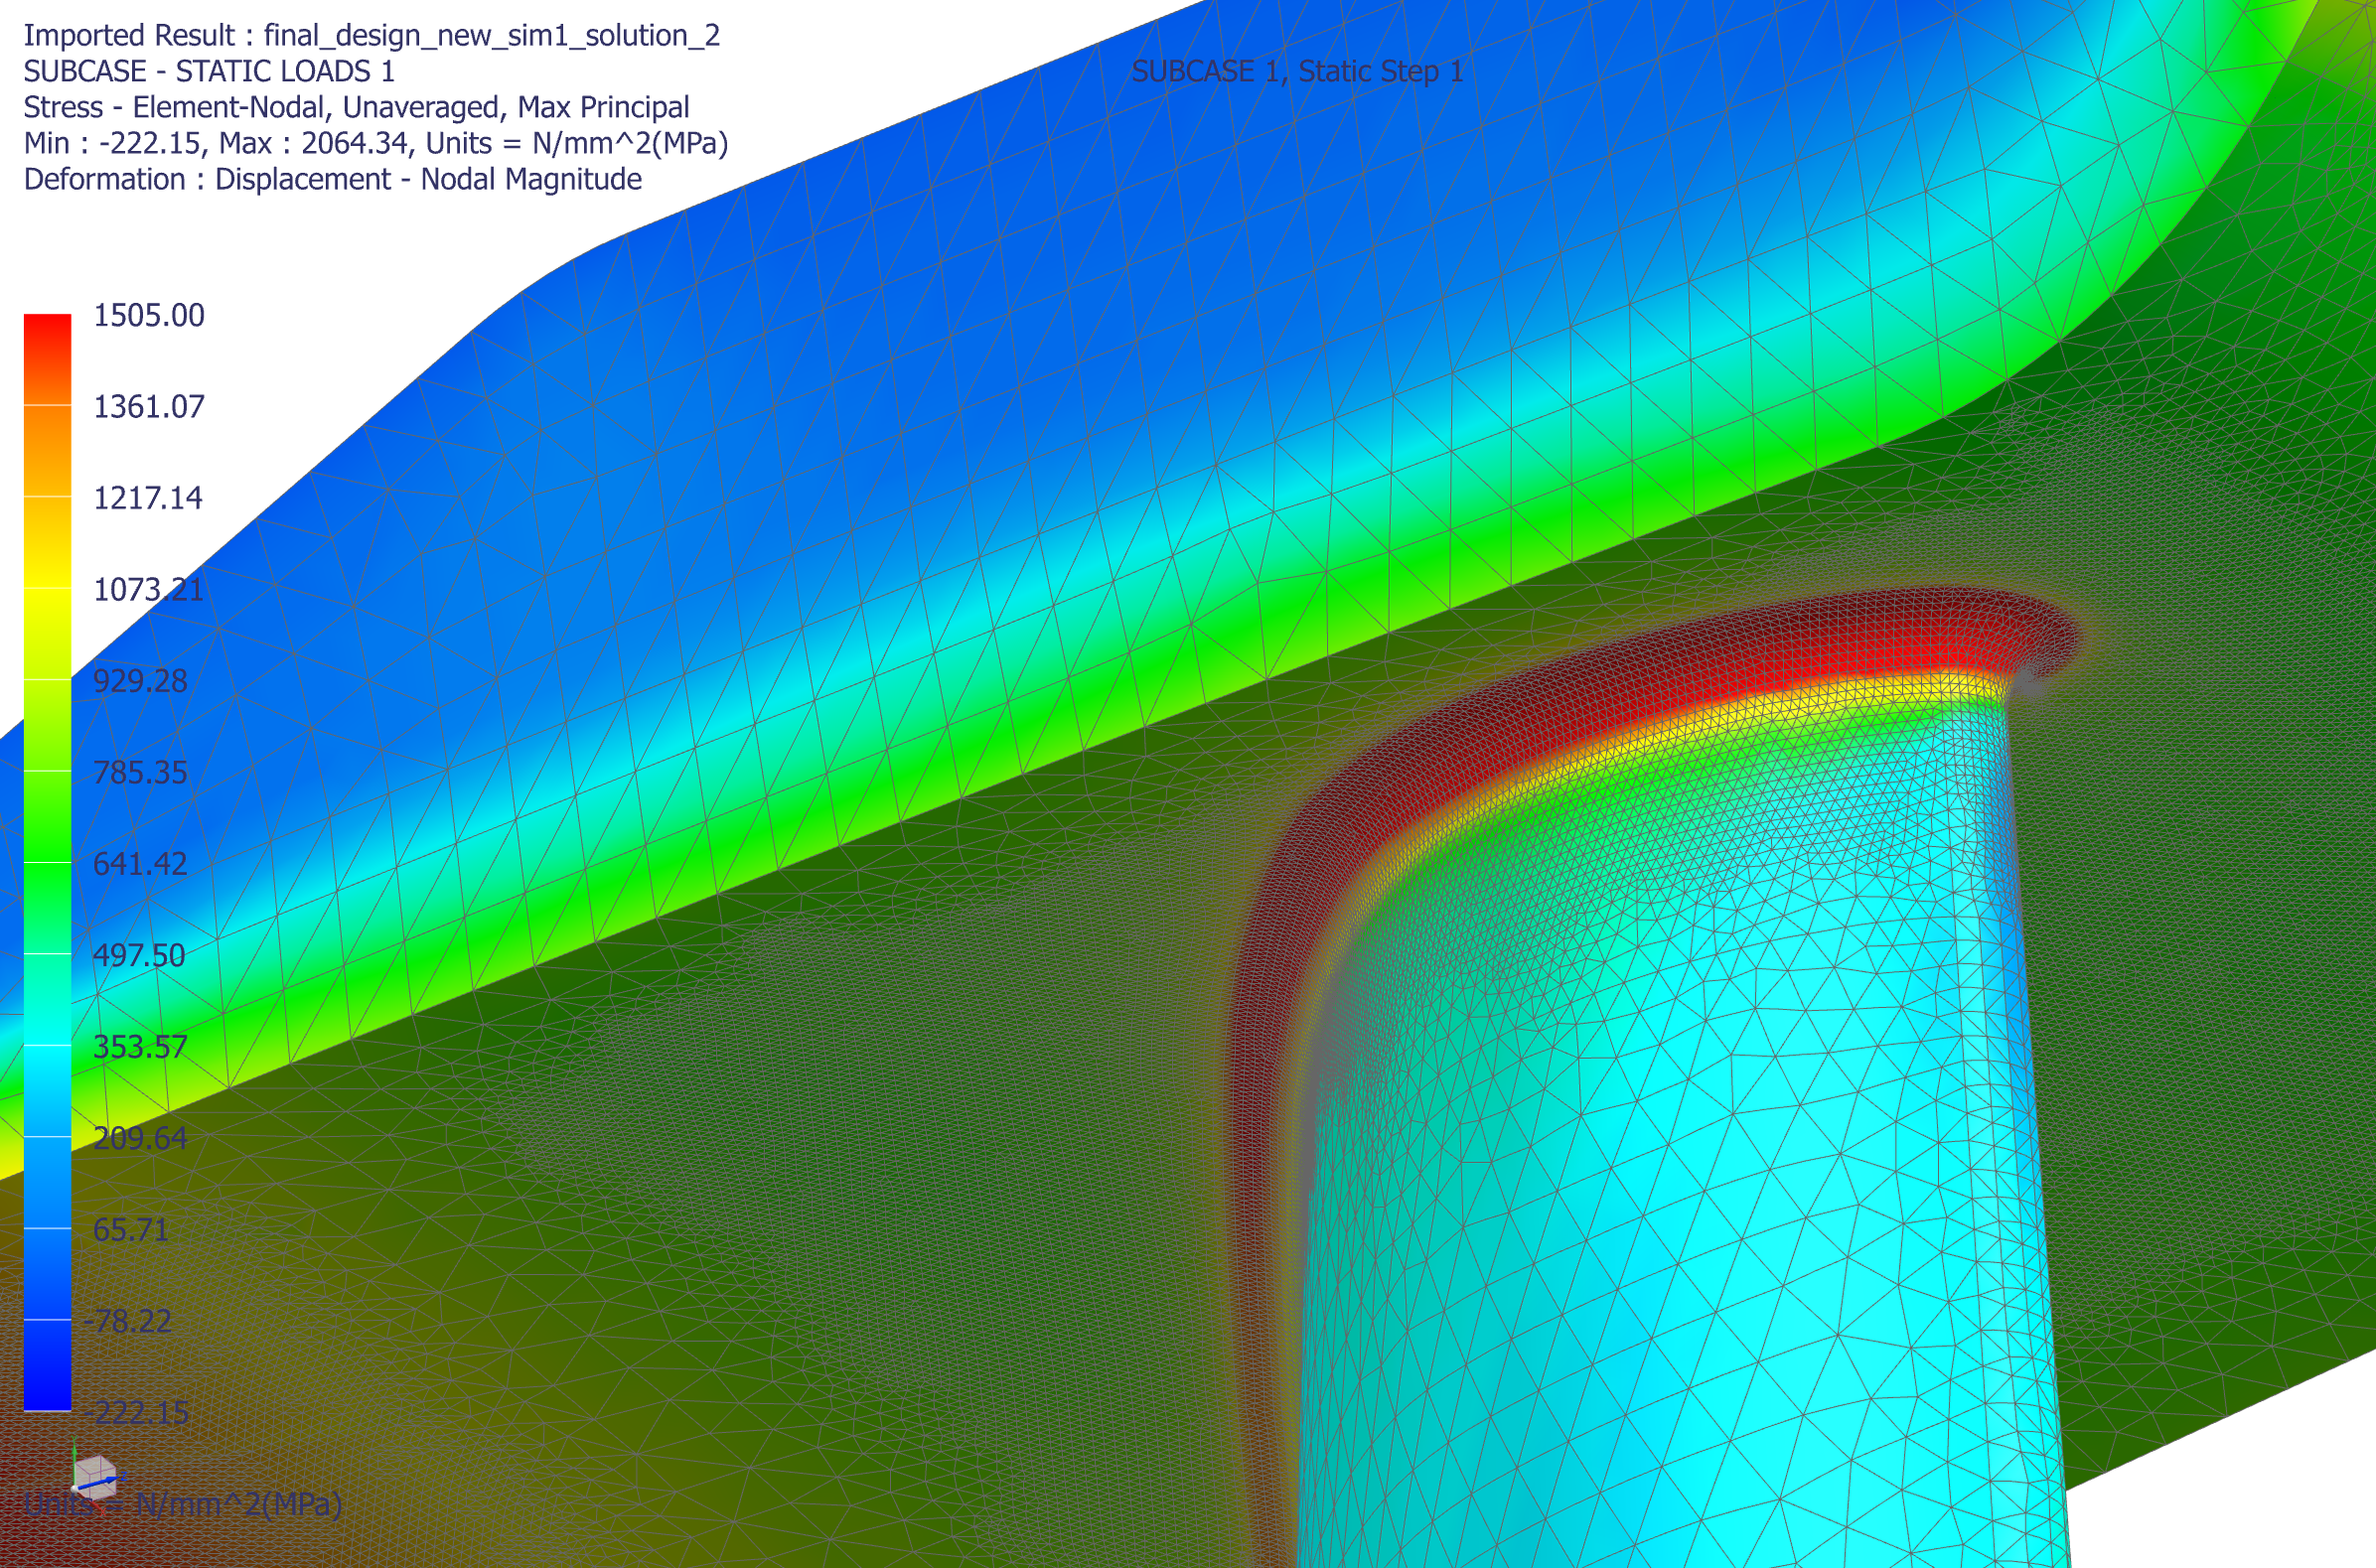
\includegraphics[width=0.7\textwidth]{Figures/finaldesign_shutdown2.png}
\caption{High stress point Shut-down condition }
\label{fig:highstressshutdown2}
\end{figure}

\begin{figure}[H]
\centering
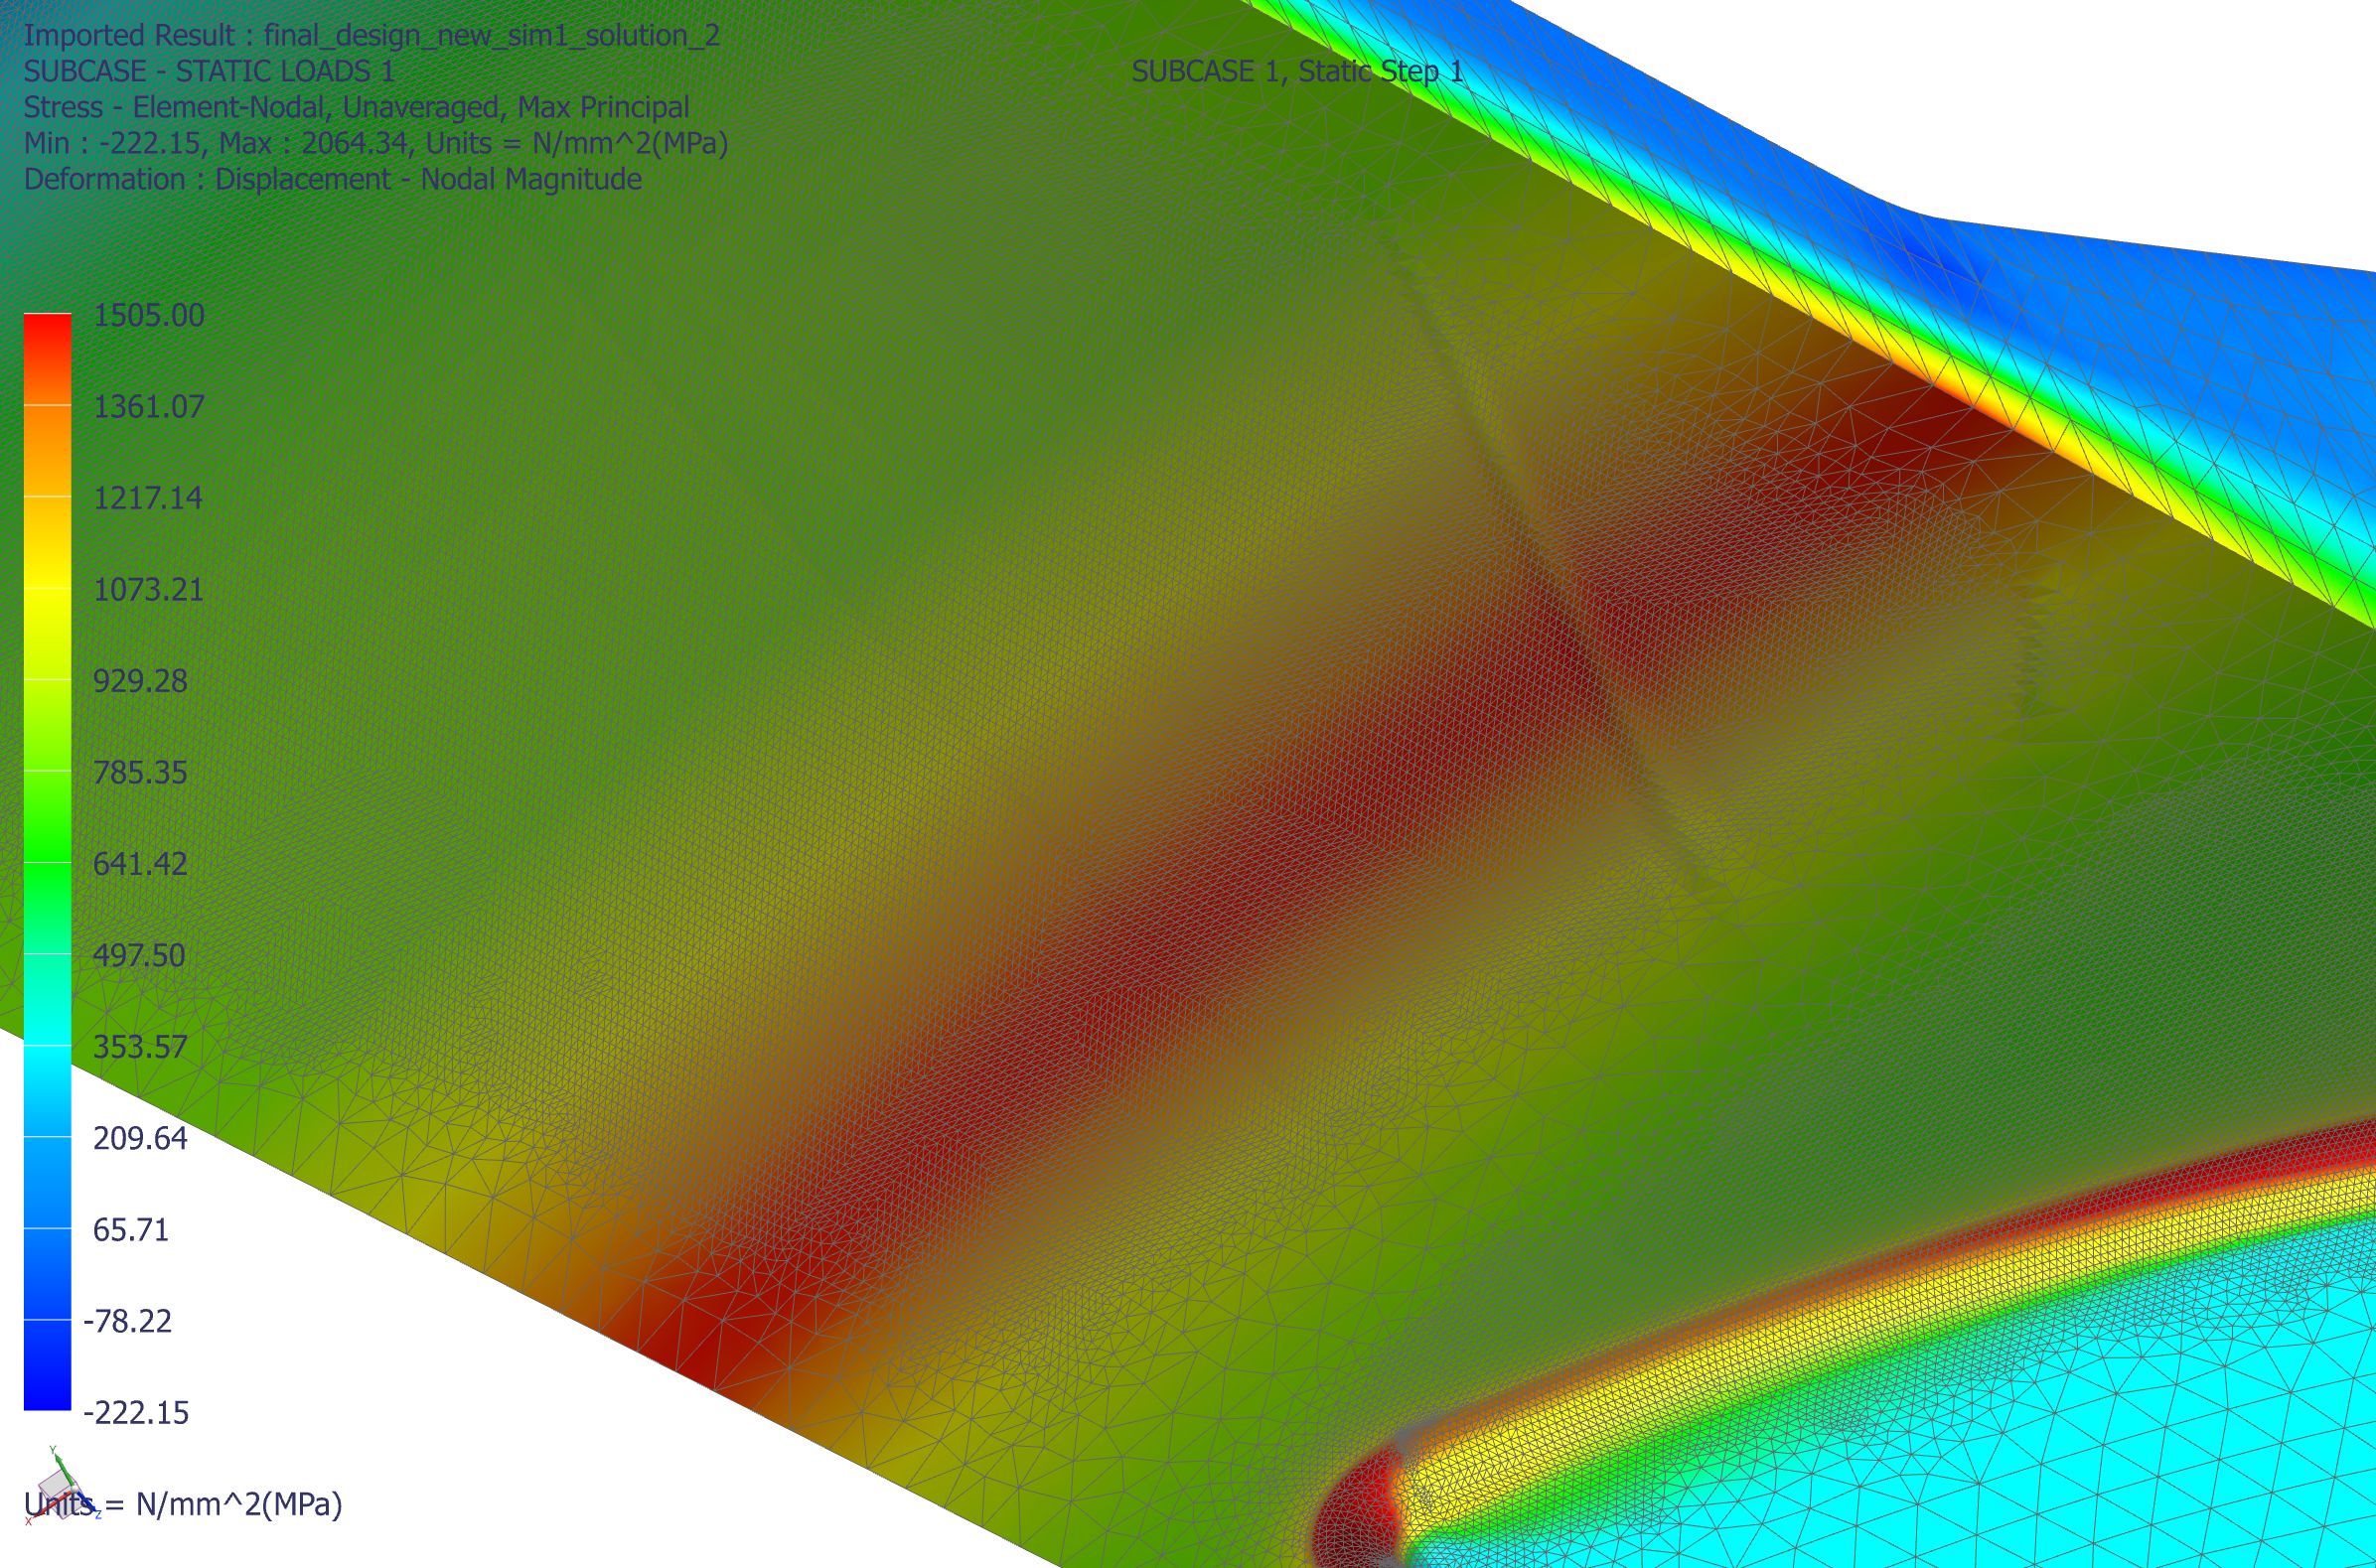
\includegraphics[width=0.7\textwidth]{Figures/finaldesign_shutdown3.png}
\caption{High stress point Shut-down condition }
\label{fig:highstressshutdown3}
\end{figure}

\subsection{Operational condition}

\begin{figure}[H]
\centering
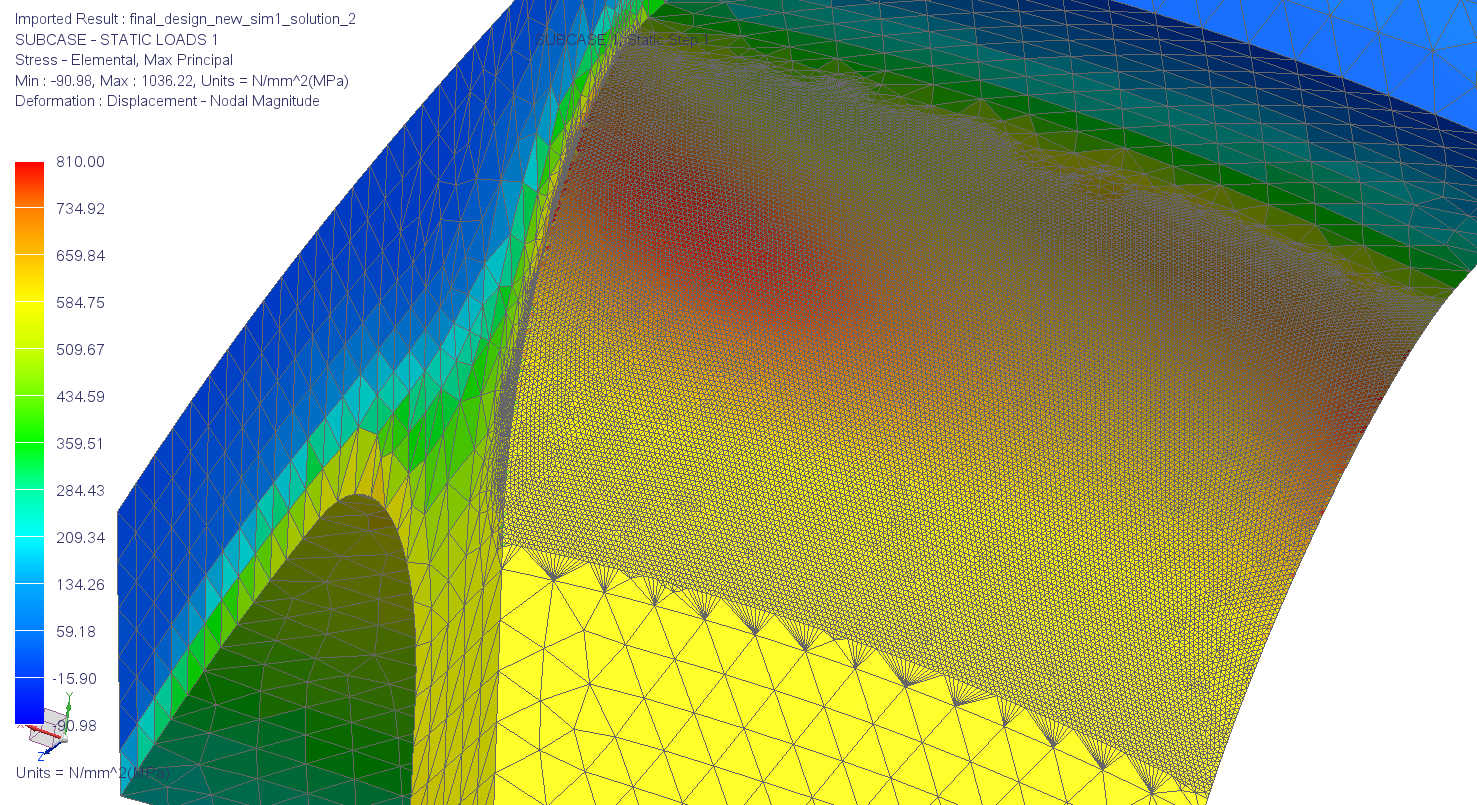
\includegraphics[width=0.7\textwidth]{Figures/Redisgn_Op_Edgeblend.png}
\caption{High stress point Operational condition }
\label{fig:highstressoperational1}
\end{figure}

\begin{figure}[H]
\centering
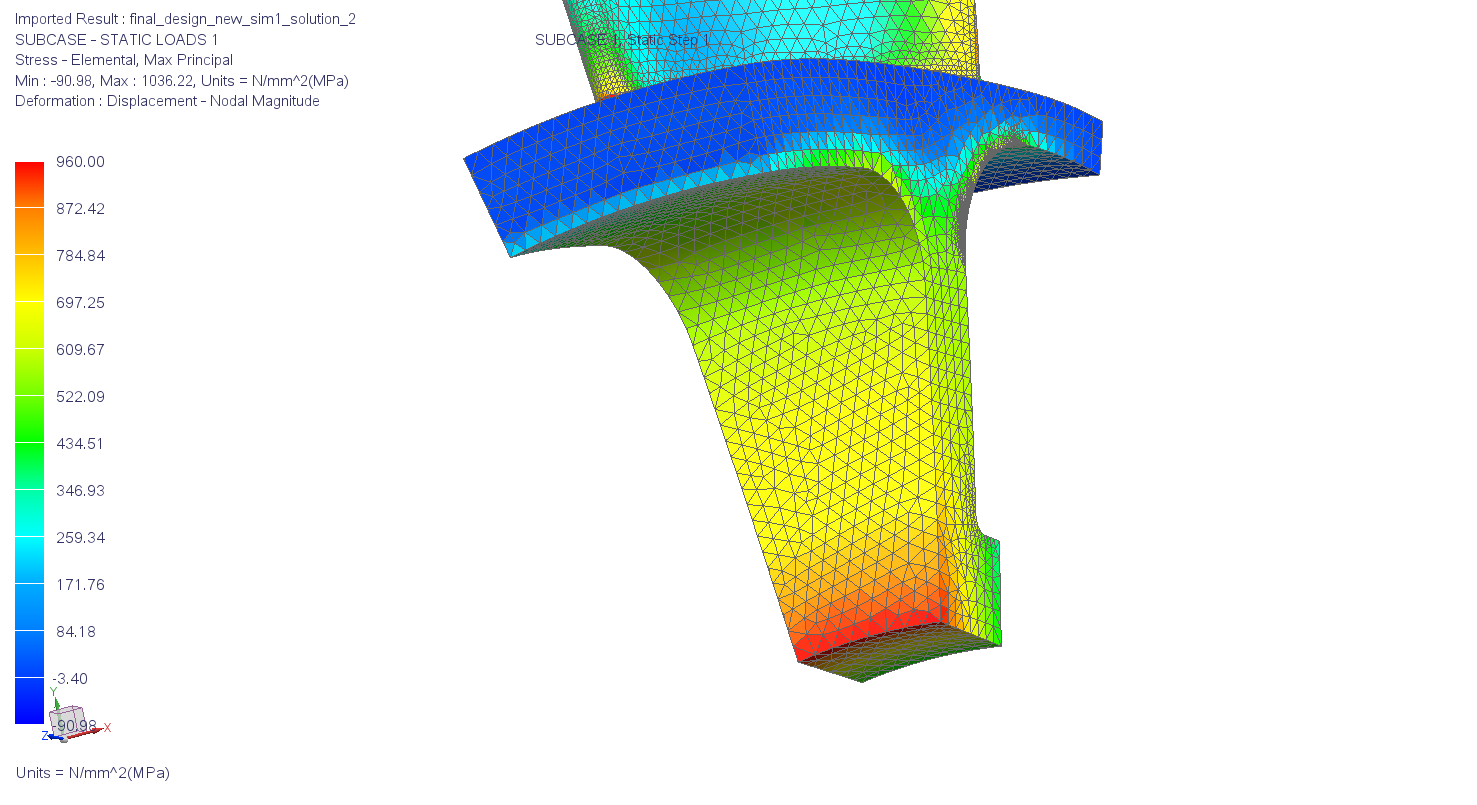
\includegraphics[width=0.7\textwidth]{Figures/Redisng_Op_Edge.png}
\caption{High stress point Operational condition }
\label{fig:highstressoperational3}
\end{figure}

\begin{figure}[H]
\centering
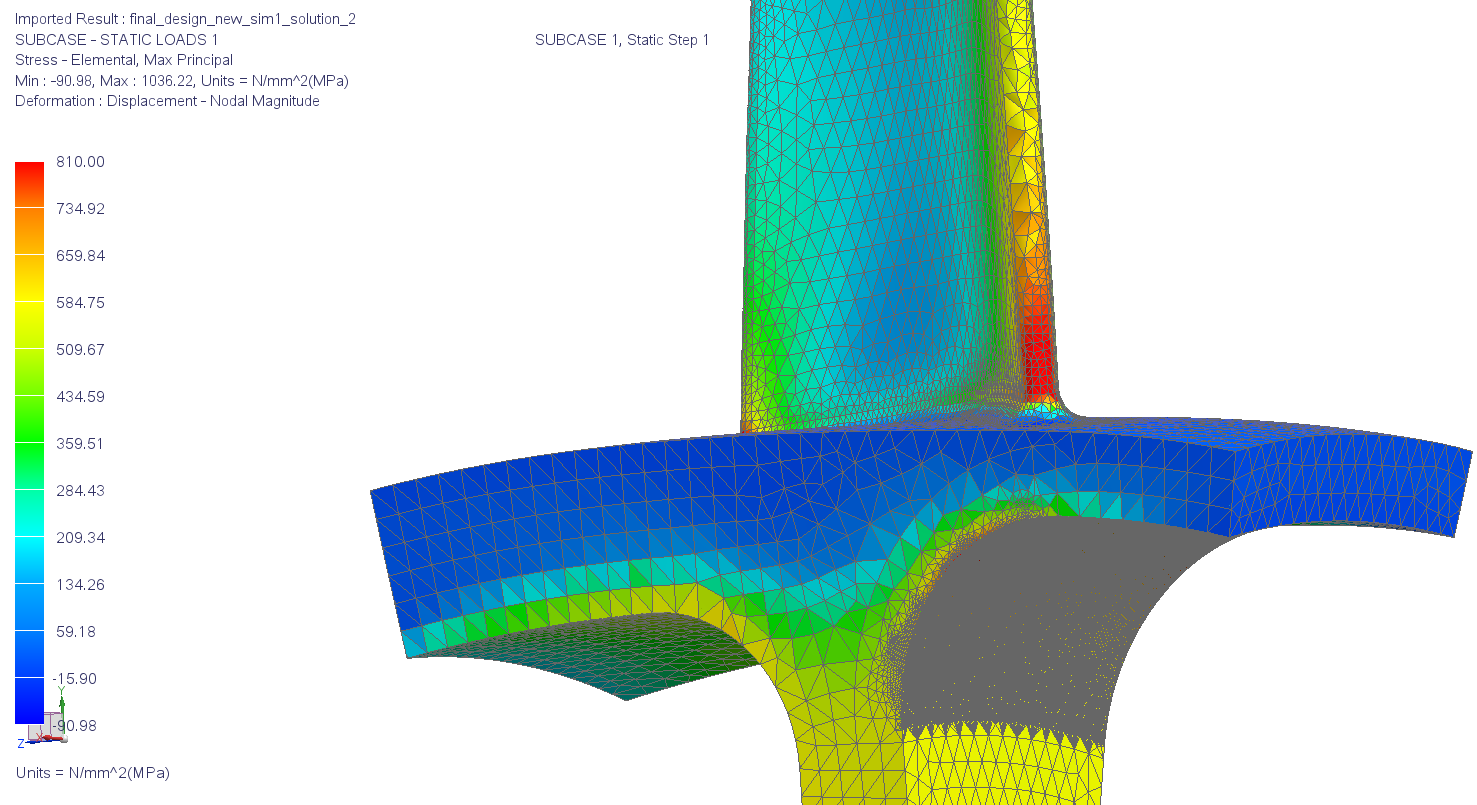
\includegraphics[width=0.7\textwidth]{Figures/Redesign_Op_Blade.png}
\caption{High stress point Operational condition }
\label{fig:highstressoperational2}
\end{figure}

\subsection{Elimination of alternative design}
\label{AppendixA3}
During the design phase a lot of changes in the case description have been made which lead to changing the re-design. Eventually, two totally different designs were left and then the 'wave' is chosen as the final design. The other design, which results during operating conditions were a little better than the wave, can be seen in Figure \ref{fig:dakje_design} below:
\begin{figure}[H]
\centering
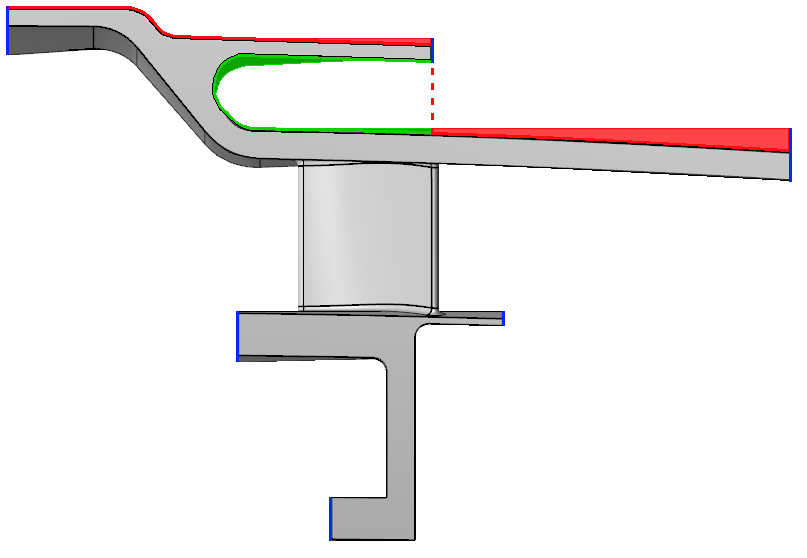
\includegraphics[width=0.7\textwidth]{Figures/dakje_design.PNG}
\caption{The alternative re-design for the stator with colour-indicated constraints. Note: Do not mind the bottom part, this is still from the original stator.}
\label{fig:dakje_design}
\end{figure}
There are three reasons for choosing the wave design over this alternative:
\begin{itemize}
\item First of all the manufacturability of the stator, which is easier for the wave design than for this alternative. For creating the hole in this stator a 'rule of thumb' of 1:3 in diameter:length must be applied to be able to manufacture this part \cite{metalcutting}. But if you look at this design and compare it with the wave design you can see that creating the top part of the stator will be easier when it comes to rounding of the edges. It is hard to round off the edges in this design because the freedom of positioning the tool is restricted to the diameter of the hole, while in the wave design the tool does have a lot of freedom to approach these edges. The manufacturable advantage of the wave design will result in a lower manufacturing time of the stator.
\item Secondly, the alternative has an effect on the compatibility and functionality of the stator. The outer surface of the alternative design is located higher than the 'wave' design, which will have an influence on the inflowing air-flow and therefore a change in functionality. The higher outer surface  of the alternative will also need a housing with a bigger radius, since the radius of the stator will also increase.
\item Lastly, the zero heat flux constraint which is applied to the green indicated surface of the alternative design. According to the 'temperature constraint (for areas inbetween)' discussion on the forum that the zero heat flux constraint can be applied to the green surface as well, along with the blue surfaces. However, this assumption has, in contrast to the blue surfaces, a big influence on lowering the stress while in reality there is heat flux in this part. This is also a reason for not choosing this alternative design, because the results of the simulation should be applicable to the reality.  
\end{itemize}
\newpage
